\section{
    Implemente no JFlap uma Máquina de Turing que, dada uma cadeia binária com ocorrências de \#’s, remova todas essas ocorrências, independentemente de suas posições
    }

\setlength{\parindent}{4em}
\setlength{\parskip}{0.5em}
\renewcommand{\baselinestretch}{1}

% \begin{figure}[h]
%     \centering
%     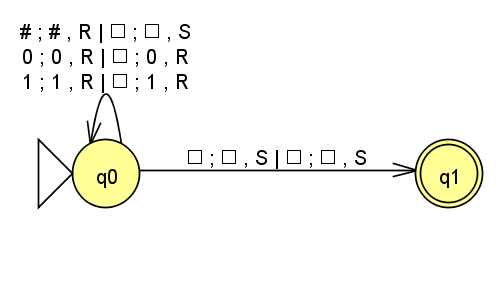
\includegraphics[width=0.65\textwidth]{mtex2.png}
%     \caption{Máquina de Turing desenvolvida para o exercício no JFlap.}
%     \label{fig:mtex2}
% \end{figure}


